\documentclass{article}
\usepackage{../../Self_Style}

\title{Phys 20AL Week 1 In Lab Notes: Pendulum}
\author{Zih-Yu Hsieh}
\date{\today}

\begin{document}
\maketitle

\section{Aim of Experiment}
The aim for this experiment is to understand how the period of a pendulum is affected by the length of the pendulum, and the mass of the pendulum.

\section{Environment Setup}
\begin{itemize}
    \item[1.] Prepare a stand and fix it at the edge of the table, and prepare a protractor that is fixed horizontally on the top of the stand.
    \item[2.] Prepare a clip and a nearly massless string, combine one end of the string to the clip and clip it onto the stand. This is used for controlling the length of the pendulum.
    \item[3.] Put the other end of the string through a hole on the top of the stand to setup a pivot for the pendulum.
    \item[4.] Hang the mass for the pendulum at the end of the string that passes through the hole in 3.
\end{itemize}
\begin{figure}[h!]
    \begin{center}
        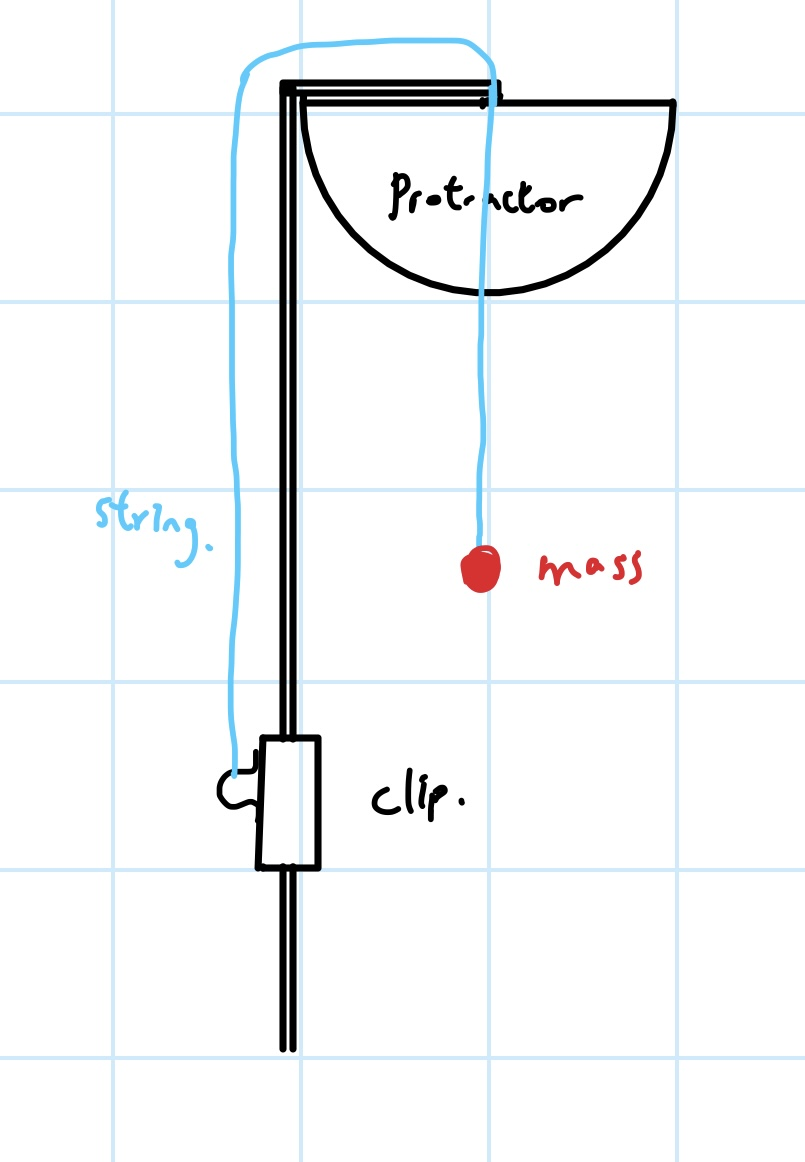
\includegraphics[width=100pt]{setup_sketch.png}
        \caption{A Drawing of the Setup}
    \end{center}
\end{figure}

\section{Measurement, and Method of Measure}
For each individual trial we'll record the length of the pendulum using tape measure or meter stick (unit: meter), use the mass scale to measure the hanged mass on the pendulum (unit: gram), and use the timer to measure the pendulum's period (unit: second).

\begin{itemize}
    \item The lengths of the pendulum used are $0.3m, 0.4m, 0.5m$, and $0.6m$. 
    \item The mass of the pendulum used are $5.5g, 20g, 66g$, and $71.5g$ (based on the provided weights). 
\end{itemize}
For the experiment, we'll follow the procedure below:
\begin{itemize}
    \item[1.] First, fix a mass for the pendulum, then fix a length for the pendulum.
    \item[2.] Raise the pendulum till it is $10^\circ$ away from equilibrium and release.
    \item[3.] Wait for the pendulum to complete $5$ cycles, then record the period for the $6^\textmd{th}$ cycle.
    \item[4.] Repeat Step 2 and 3 five times, with fixed mass and length.
    \item[5.] Change the length of the pendulum, and repeat Step 2 to 4 for each desired length.
    \item[6.] Change the mass of the pendulum, and repeat Step 2 to 5 for each desired mass.
\end{itemize}
Here, the idea is to first measure the affect of different lengths on the period of the pendulum when fixing the mass, then repeat similar process for each chosen mass.

\section{Data and Uncertainties}
\begin{figure}[h!]
    \begin{center}
        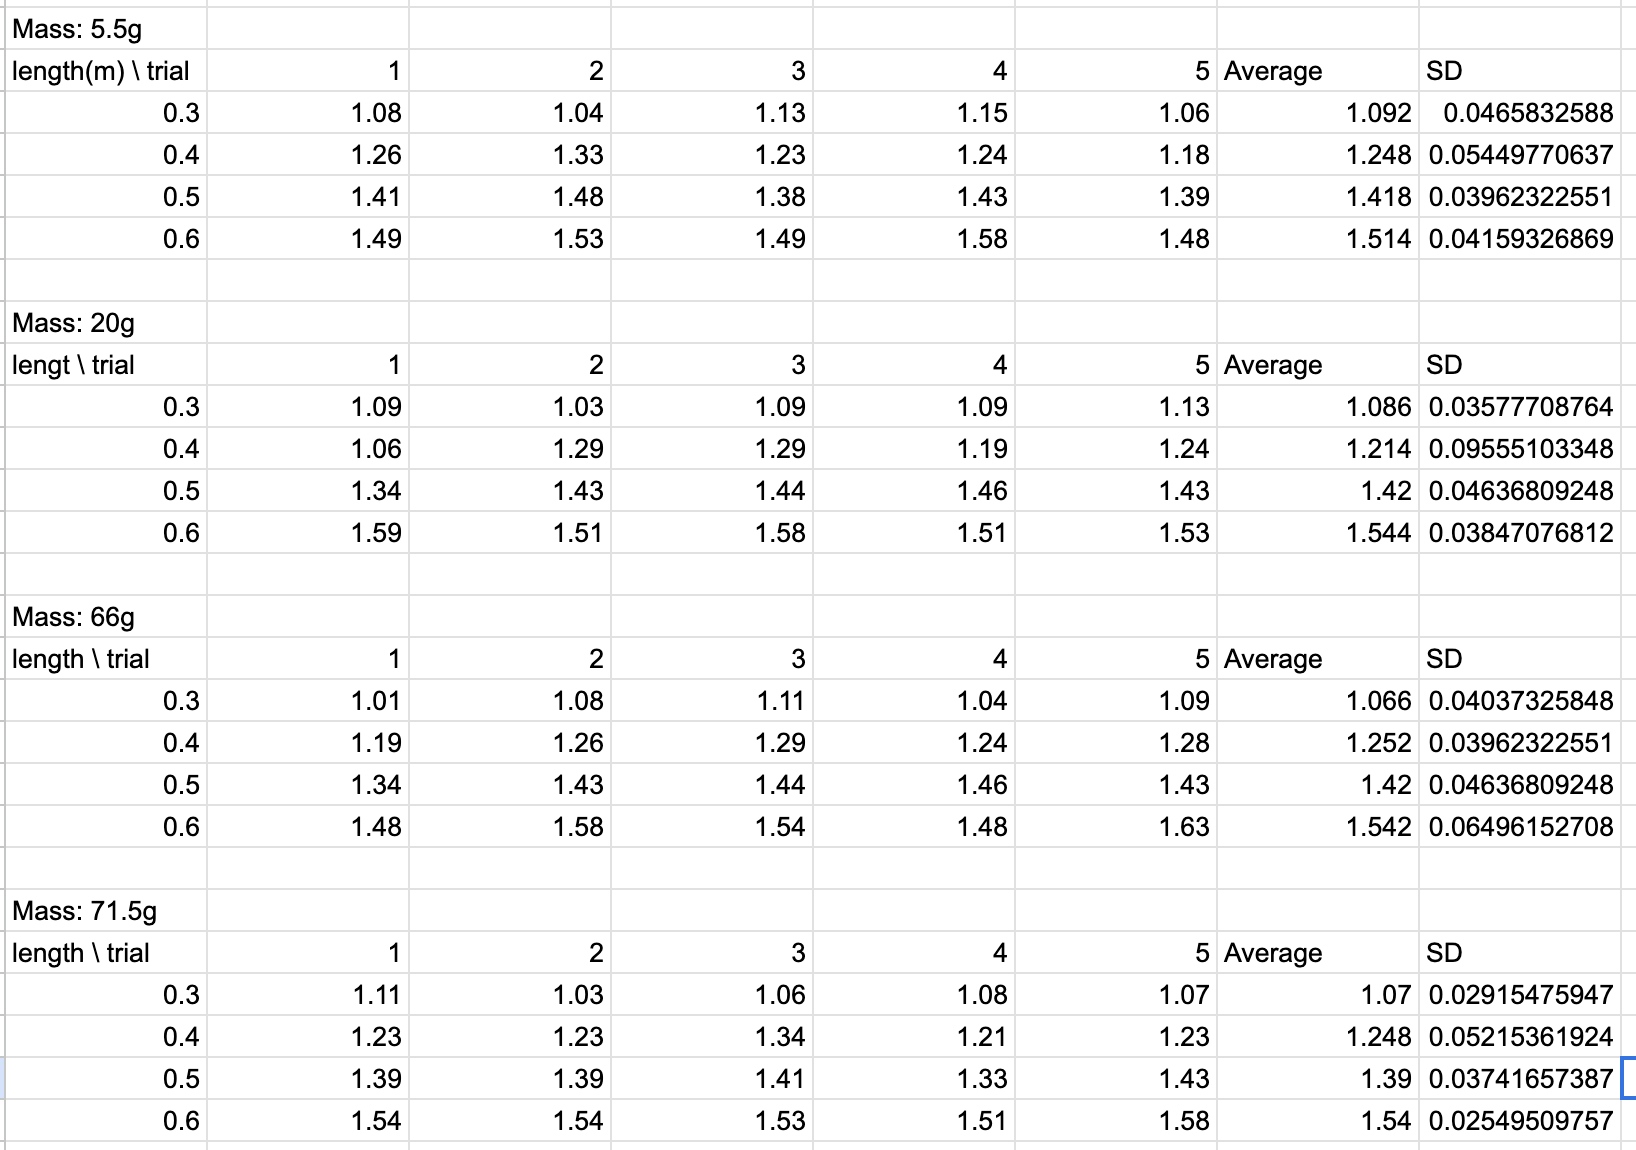
\includegraphics[width=150mm]{data.png}
    \end{center}
\end{figure}
Some uncertainties (or sources of error) observed during the experiment includes: Air Resistence, error when doing measurement with raw eyes (when measuring length and angle of the pendulum), and Human's reaction time (when clicking the timer).

\end{document}